\begin{frame}
    \frametitle{Die blineare Differenzialform}
    \begin{itemize}
        \item Jeder Transformation lässt bestimmte Größen unverändert
        \item Diese Invarianten bestimmen Eigenschaften der Transformation
        \item Für kanonische Transformation hatten wir zunächst $\sum p_i \delta q_i$
        \item Dann fanden wir die allgemeinere Bedingung     
                \begin{displaymath}
                \sum_{i=1}^{n} (p_i \delta q_i - P_i \delta Q_i) = \delta S
                \end{displaymath}
              Welcher Invarianten entspricht diese Bedingung?
    \end{itemize}
\end{frame}

\begin{frame}
   
        \begin{displaymath}
        \sum_{i=1}^{n} p_i \delta q_i - \sum_{i=1}^{n} P_i \delta Q_i = \delta S
        \end{displaymath}
        
        $\longrightarrow$ Erinnert an die Arbeit in einem monogenen (monogenic) System.\\
        \vspace{3mm}
        \emph{Masseteilchen wird auf beliebigem geschlossenen Pfad bewegt.\
              Ist die verrichtete Arbeit Null, wenn man wieder am Ausgangspunkt ankommt, so nennt man das System monogen.}
            
      \begin{center} 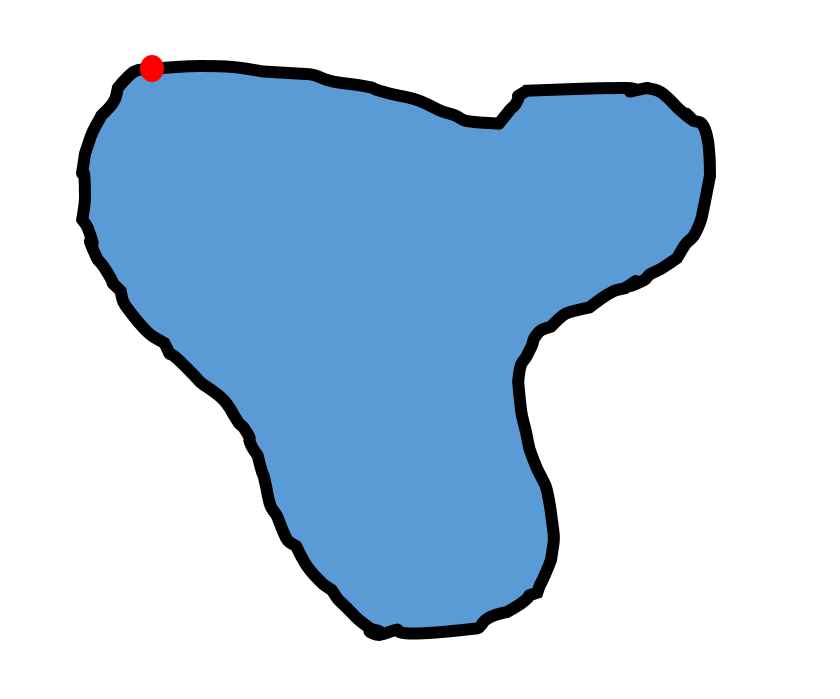
\includegraphics[scale=0.15]{images/monogenicSys}  \end{center}  
        
        

\end{frame}

\begin{frame}
    Integration von
    \begin{displaymath}
    \sum_{i=1}^{n} p_i d q_i - \sum_{i=1}^{n} P_i d Q_i = d S
    \end{displaymath}
    entlang einer geschlossenen Kurve ergibt:
   \begin{displaymath}
   \oint \sum_{i=1}^{n} p_i d q_i - \oint \sum_{i=1}^{n} P_i d Q_i = 0
   \end{displaymath}
    \begin{center} 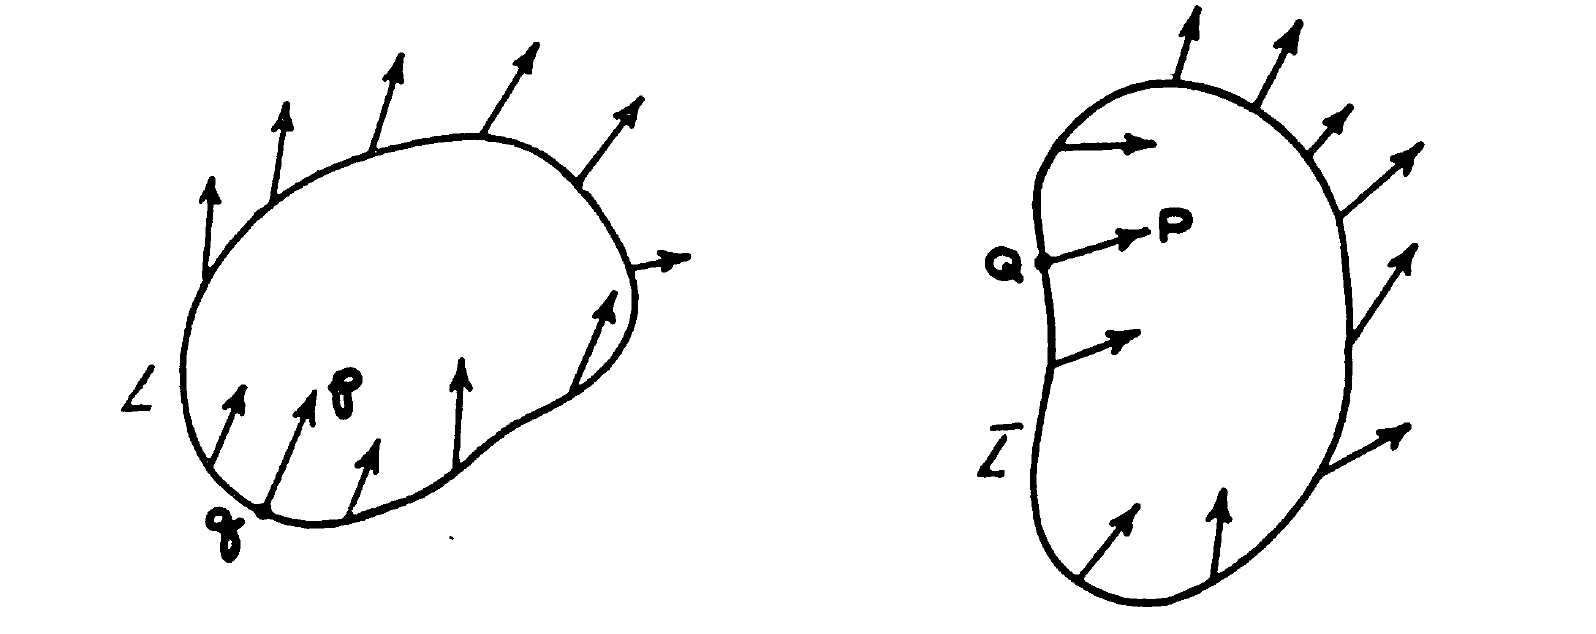
\includegraphics[scale=0.225]{images/circulation}  \end{center}  

\end{frame}

\begin{frame}
     \emph{Für jede geschlossene Kurve im Phasenraum ist}
    \begin{displaymath}
    \Gamma = \oint \sum_{i=1}^{n} p_i d q_i = \oint \sum_{i=1}^{n} P_i d Q_i
    \end{displaymath}
     \emph{eine Invariante gegenüber der kanonischen Transformationen.}
 
\end{frame}